% Auth: Nicklas Vraa
% Docs: https://github.com/NicklasVraa/LiX

\documentclass{textbook}
\usepackage{graphicx}
\usepackage{subcaption}
\usepackage{float}

\hypersetup{
    colorlinks=true,
    linkcolor=blue,
    filecolor=magenta,      
    urlcolor=blue,
    pdftitle={Overleaf Example},
    pdfpagemode=FullScreen,
    }
    
\lang      {english}
\title     {Kentech Tutorial of Advancing Sustainability through Computational Chemistry Methods}
% \subtitle  {Kentech CCP 2023 Summer - Let's Roll a Dice: Monte Carlo Simulation 101}
\author     {EF KENTECH Chemistry}
\date       {\today}
% \cover*    {resources/textbook_front.png}{resources/textbook_back.pdf}
% \license   {CC}{by-nc-sa}{3.0}{The Company}
% \isbn      {978-0201529838}
% \publisher {JK}
% \edition   {Summer}{2023}
% \dedicate  {Kentech Community}{JK}
% \thank     {JK}
% \keywords  {computational chemistry, Monte Carlo}
% \note{JK}
% \maketitle
\begin{document}

\h*{Kentech Tutorial of Advancing Sustainability through Computational Chemistry Methods} %Non-Numbered Heading
In today's advancing landscape of science and engineering,  computational methods have become an essential tool. With the advent of artificial intelligence and machine learning, their importance is only further heightened, where they are increasingly being used to make groundbreaking discoveries and advances.

This tutorial is a collaborative effort that showcases the work of undergraduate students of Kentech, with a focus on the computational elements of Chemistry and Engineering. This document will be updated on a regular basis, reflecting the ongoing learning and innovative activities taking place at Kentech.

Yet, this tutorial is more than just a collection of academic activities. It is envisaged as a platform facilitating the exchange of knowledge and experiences amongst students. Through such discourse, I aspire to foster a positive and dynamic learning culture at Kentech. As we navigate this path of scientific exploration, we are committed to learning, sharing, and collectively evolving.

In the spirit of collaboration, all developed codes will be shared openly via GitHub, further enriching the learning experience and ensuring an open-source approach to our scientific journey.

August 6, 2023

Jeongmin Kim (and ChatGPT-4)

\toc
\h{Monte Carlo Simulation 101}
This chapter was developed through a CCP program entitled "Let's Roll a Dice: Monte Carlo Simulation 101" with the support of Kentech Residential College Education Center.
All the codes are available at \url{our GitHub page}{https://github.com/Jeongmin0658/kentech_tutorial}. \textcolor{magenta}{JK: this page is still private.}

\textcolor{red}{\textbf{To-Do List}:
    \begin{itemize}
        \item Front and Back cover pages - photos that summarize our activities
        \item Contributors: Insert your photo, self-introduction, and experience in CCP this summer at your fav position.
    \end{itemize}
}

\hh{Editorial}
Page for our Editor, Seohyun Kim.

\hh{Contributors}
\begin{figure}[H]
  \centering
    \begin{minipage}{0.9\textwidth} % Set the width of the entire figure here
  \begin{subfigure}{0.3\textwidth}
    \includegraphics[width=\textwidth]{example-image-a}
    \caption{Contributor A1}
  \end{subfigure}
  \hfill
  \begin{subfigure}{0.3\textwidth}
    \includegraphics[width=\textwidth]{example-image-b}
    \caption{Contributor A2}
  \end{subfigure}
  \hfill
  \begin{subfigure}{0.3\textwidth}
    \includegraphics[width=\textwidth]{example-image-c}
    \caption{Contributor A3}
  \end{subfigure}
  
  % You can add some vertical space in between the rows
  \vspace{1cm}

  % The next row
  \begin{subfigure}{0.3\textwidth}
    \includegraphics[width=\textwidth]{example-image-a}
    \caption{Contributor B1}
  \end{subfigure}
  \hfill
  \begin{subfigure}{0.3\textwidth}
    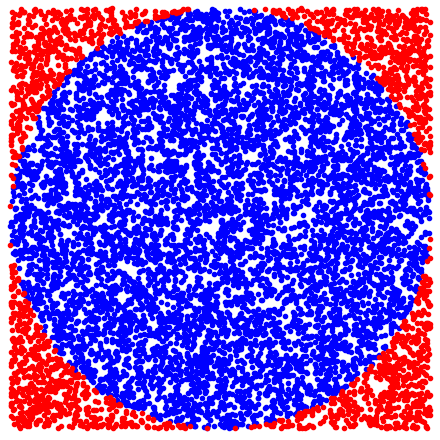
\includegraphics[width=\textwidth]{resources/textbook_front.png}
    \caption{Contributor B2}
  \end{subfigure}
  \hfill
  \begin{subfigure}{0.3\textwidth}
    \includegraphics[width=\textwidth]{example-image-c}
    \caption{Contributor B3}
  \end{subfigure}

    % You can add some vertical space in between the rows
  \vspace{1cm}

  % The next row
  \begin{subfigure}{0.3\textwidth}
    \includegraphics[width=\textwidth]{example-image-a}
    \caption{Contributor C1}
  \end{subfigure}
  \hfill
  \begin{subfigure}{0.3\textwidth}
    \includegraphics[width=\textwidth]{example-image-b}
    \caption{Contributor C2}
  \end{subfigure}
  \hfill
  \begin{subfigure}{0.3\textwidth}
    \includegraphics[width=\textwidth]{example-image-c}
    \caption{Contributor C3}
  \end{subfigure}

  \caption{Contributors of 2023 summer edition}
  \end{minipage}
\end{figure}

\hh{Basics 1: GitHub and Google CoLab}
This part is about how to use GitHub and CoLab. Should be very practical
Byungchan, June, Suhyun
\textcolor{magenta}{JK: Again, should be very practical. Anyone can use both tools if they follow what's illustrated in this section.}

\hh{Basics 2: Latex and Overleaf}
This part is about how to use overleaf and Latex. Should be very practical as well. Maybe include the Usages below.
\textcolor{magenta}{JK: This might not be part of this summer edition.}


\hh{Scientific coding with Python}
This part contains the activity of the first meeting.
Minyong, Eunseo, Seojin
\textcolor{magenta}{JK: better to introduce simple Python statements such as for-statement, if-statement, etc.}

\hh{Pi estimation}
This part contains the activity of the second meeting.
Seohyun, Gahyun
\textcolor{magenta}{JK: Introduce an idea where how we compute Pi numerically, and one method is Monte Carlo.}

\hh{Ising model}
This part contains the activity of the third meeting.
Hansu, Jisu


\h{Us.ages - Will be deleted}
Heading

\hh{Subheading}
Subheading

\hhh{Subsubheading}
Subsubheading

\hh{Formats}
Nunc ante \b{bold} lectus, pretium id \i{italic} sodales, dapibus \s{strikethrough} urna. Suspendisse maximus \u{underlined} metus sed ante commodo efficitur. Some inline code: \c{def func(a,b): return a+b}

\hh{Mathematics}
Pellentesque sagittis orci ut lorem blandit, vel cursus urna interdum. Mauris malesuada fermentum ipsum, accumsan varius velit porttitor ut. Lorem ipsum dolor sit amet, consectetur adipiscing elit. Etiam rutrum sem orci, eget ornare justo sodales.

    \math{my_equation}{\hat{x}_i = \frac{x_i-\mu}{\sqrt{\sigma^2+\epsilon}}}

\hh{Code Blocks}
Nullam congue ligula vitae urna convallis commodo. Proin nunc mi, vulputate quis viverra eu, consequat vitae risus sed venenatis. Praesent ut libero in dui mattis maximus.

    \code{my_code}{python}{
    # You Learned Python Today.

    if num == 1:
      print(num, "is not a prime.")
    elif num > 1:
      for i in range(2, num):
        if (num % i) == 0:
          print(num, "is a prime.")
          break
    }
    {This is some code.}

Cras vitae sem egestas, elementum felis vitae, ultricies ante. Fusce pellen tesque massa vitae massa molestie, at cursus urna scelerisque. Aliquam malesuada nunc at est vulputate condimentum. Cras fermentum nisi sit amet nulla pulvinar, vel vulputate ante tempor. Quisque vehicula nibh tortor, nec consectetur lorem semper sit amet.

\hh{Tables}
Interdum et malesuada fames ac ante ipsum primis in faucibus. Pellentesque eget mauris vitae metus pulvinar hendrerit nec non metus. Sed bibendum sapien non elit tempus accumsan. Phasellus in leo eu dui auctor laoreet. Etiam dui tellus, congue consequat accumsan nec, condimentum at est.

    \tabs{my_table}{cols}{
    This & is & a & cool & table \\
    1    & 2  & 3 & 4    & 5     \\
    a    & b  & c & d    & e     \\
    }
    {This is a table - Notice that the description wraps.}

\hh{Figures}
Nullam massa nunc, sollicitudin id eleifend vitae, pellentesque sit amet lectus. Morbi vestibulum leo quis tempor lacinia. Praesent vitae est ante. Fusce dignissim in urna et posuere.

    \fig{my_svg}{0.3}{resources/placeholder.svg}
    {This is an svg-figure scaled by 0.3, and this is a very long description.}

Integer sed metus malesuada, volutpat urna condimentum, aliquet metus. Phasellus interdum.

\hh{Lists}
Elit vel sagittis luctus, arcu libero pellentesque nisi, sed consectetur quam neque a elit. Donec consectetur cursus nulla eu feugiat. Lorem ipsum dolor sit amet, consectetur adipiscing elit.

    \items{
    ¤ Something.
    ¤ Another thing.
        \items{
        ¤ A subitem.
        ¤ Another subitem.
            \items*{
            ¤ A subitem.
            ¤ Another subitem.
            }
        }
    ¤ And another item.
    ¤ Last item.
    }

Pellentesque et blandit leo. Sed lacinia, sapien sit amet posuere tempor, eros nunc consectetur massa, id pulvinar diam nulla ut felis. Nam id iaculis dui. Pellentesque dapibus, ligula non gravida euismod, risus odio feugiat quam, id ultrices tellus est et dui.

\hh{Referencing}
Here is a hyperlink to a \url{webpage}{https://www.overleaf.com/}. This is a reference to \r{my_equation}, and this refers to \r{my_svg}. You can also refer to headings like \r{Tables}. \R{my_code} is a capitalized variant. For all references, both the name and number are links.

\end{document}
